\section{微分方程的离散化}

对于不容易求解的微分方程,比如高阶方程,可以通过对时间的离散化变成差分方程,再通过递归获得数值解。

本节要点:
\begin{itemize}
    \item 掌握欧拉近似方法。
\end{itemize}

%============================================================
\subsection{一阶微分方程的欧拉近似}

一阶常系数微分方程:
\[
\frac{dy}{dt}+Py=Qx \qquad t\geqslant t_0
\]
假设时间取离散点$t=nT$,则:
\[
\frac{dy\left( nT \right)}{d\left( nT \right)}+Py\left( nT \right) =Qx\left( nT \right) \qquad n=0,1,2,\cdots
\]
如果采样周期足够小,方程左边可以认为$\frac{1}{T}\left[ y\left( nT+T \right) -y\left( nT \right) \right] +Py\left( nT \right) $,于是一阶微分方程可以离散地表示为:
\[
y\left[ n \right] +\left( PT-1 \right) y\left[ n-1 \right] =TQx\left[ n-1 \right] \qquad n=0,1,2,\cdots
\]
该一阶差分方程即为一阶微分方程的近似,根据之前讨论的方法即可得到采样点的输出信号,该过程称为{\bf 欧拉近似}(Euler approximation)。
欧拉近似是一种对微分方程数值化求解的方法,采样周期越小,精度越高。

%============================================================
\subsection{二阶微分方程的欧拉近似}

对于二阶微分方程:
\[
\frac{d^2y}{dt^2}+A_1\frac{dy}{dt}+A_0y=B_1\frac{dx}{dt}+B_0x \qquad t\geqslant t_0
\]
用欧拉近似可得差分方程:
\begin{align*}
&\frac{y\left[ n \right] +y\left[ n-2 \right]}{T^2}+A_1\frac{y\left[ n-1 \right] -y\left[ n-2 \right]}{T}+A_0y\left[ n-2 \right] \\
&=B_1\frac{x\left[ n-1 \right] -x\left[ n-2 \right]}{T}+B_0x\left[ n-2 \right]
\end{align*}
整理后:
\begin{align*}
&y\left[ n \right] +\left( A_1T-2 \right) y\left[ n-1 \right] +\left( A_0T^2-A_1T+1 \right) y\left[ n-2 \right] \\
&=B_1Tx\left[ n-1 \right] +\left( B_0T^2-B_1T \right) x\left[ n-2 \right]
\end{align*}

%============================================================
\subsection{例RC电路}

\begin{example}
以下图为例,假设电路零状态,$x\left( t \right) =1\mathrm{V},R=1\Omega ,C=1\mathrm{F}$,分别用微分方程和差分方程计算系统在0~10s这段时间内的输出。
\end{example}

\begin{figure}[h]
\centering
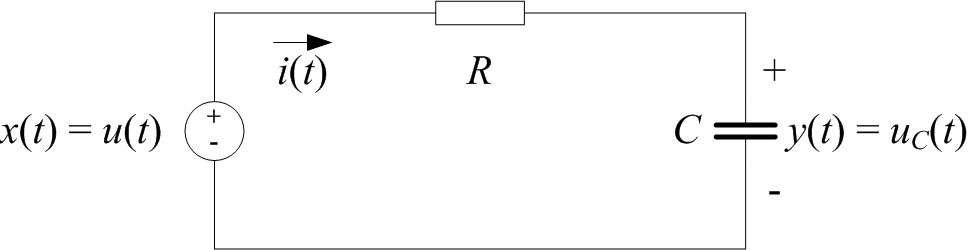
\includegraphics[height=2cm]{1.5.1-1.png}
\end{figure}
\[
\frac{dy}{dt}+\frac{1}{RC}y=\frac{1}{RC}x \qquad \begin{cases}
	x\left( t \right) =u\left( t \right)\\
	y\left( 0^- \right) =0\\
\end{cases}
\]

将之前的结果解得到输出信号并将其做欧拉近似得到差分方程:
\begin{align*}
&y\left( t \right) =1-e^{-\frac{t}{RC}}=1-e^{-t} \qquad t\geqslant 0 \\
&y\left[ n \right] +\left( T-1 \right) y\left[ n-1 \right] =Tx\left[ n-1 \right] \qquad n=0,1,2,\cdots
\end{align*}
令采样间隔$T=0.2\mathrm{s}$,微分方程和差分方程结果如下。

\begin{python}
T  = 0.2
An = np.array([T-1])
Bm = np.array([T])
b  = 0
Yn = np.array([0])
Xm = np.array([0])
t  = np.arange(0, 10, T)
X  = np.ones_like(t)
Y_differential = 1 - np.exp(-1*t)
Y_difference   = my_diff(An, Yn, Bm, Xm, b, X)

ax.plot(t, Y_differential,      label='differential')
ax.plot(t, Y_difference,   'o', label='difference')
\end{python}

\begin{figure}[h]
\centering
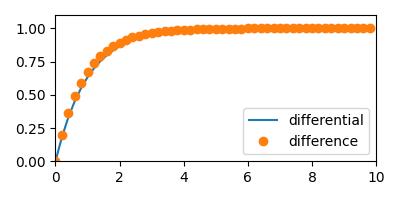
\includegraphics[height=3cm]{2.3.3-1.png}
\end{figure}




